\section{Experiments}
\label{sec:experiments}
%\TODO { Comparing with other's aspect extraction results, 
%for example using the human annotated feature words. }
%
%\TODO { Measure the semantic similarity between our extracted top aspect words 
%and the groundtruth aspects. 
%For example, find K nearest neighbors of our extracted aspect words, 
%when K=3, K=5, K=10, how many percent of the groundtruth aspects are matched?
%}
%
%\TODO { End to end aspects summarization, other's results ? }

In this section, we present the results of three experiments. 
The first one is a comparison of methods for obtaining sentence vectors. 
In the first step of our framework, i.e., sentence clustering, 
sentence representation is crucial to the performance 
and hence critical to overall framework. 
In particular, we need a vector representation 
that accurately captures the semantic similarity between sentences, 
so we test the performance of the methods on a sentence similarity 
prediction task. 
The second experiment is the comparison of our framework
with a number of baselines including the state-of-the-art approaches
in the end-to-end aspect extraction task.
The third experiment is a complete aspect-based summarization application using our model.

\subsection{Experiment 1: Comparison of Sentence Vectors}

The vector representation of sentences is a vital module of our framework, this experiment compares two models: long short-term memory (LSTM) and paragraph vector (PV). 

Since we use the sentence vectors for clustering the sentences based on 
their topics, and k-means algorithm uses the distances between the 
vectors to determine which cluster each sentence belongs to, 
we need the sentence vectors to accurately capture the semantic distance 
between the sentences. 
For this purpose, we evaluate the models using
a sentence similarity prediction task, namely the English subtask of 
SemEval-2015 Task 2: Semantic Textual Similarity \cite{agirrea2015semeval}.
There are 14,250 data entries, 11,250 for training and 3000 for test,
each containing a pair of sentences and a score from 0-5 rating 
the semantic similarity of the two sentences.
We train our models on all the sentences and 
test on the 3000 sentence pairs from the test set.

For each sentence pair, both neural network models give us the 
independent 300-dimensional sentence vectors; to use this pair of vectors to 
predict the semantic similarity, we train an independent predictor backend.
The backend is a three-layer feed-forward neural network.
It takes the two vectors for the sentence pair given by LSTM or PV as input.
The input layer takes the concatenation of the two 300-dimensional vectors;
the hidden layer is 100-dimensional; 
the output layer is a 6-class softmax, corresponding to the scores of 0 to 5;
the loss function is categorical cross-entropy.
The backend is trained independently for both LSTM and PV, 
with the same input dimensionality and network structure, 
and for the same number of iterations. 
To put our results in context, we also include the results of 
the winning system of SemEval-2015 task 2, DLS@CU \cite{dlscu}. Note that
DLS@CU doesn't use sentence vectors and cannot be used in our framework.
The results are shown in \tabref{table:semeval}.

\begin{table}
	\centering
	\caption{Pearson correlation scores on 5 parts of the test set and the mean scores.}
	\label{table:semeval}
	\begin{tabular}{|l|c|c|c|c|c|c|}
		\hline
		Model & Test 1 & Test 2 & Test 3 & Test 4 & Test 5 & Mean \\ \hline\hline
		LSTM  & 0.5717 & 0.6329 & 0.6015 & 0.7961 & 0.8147 & 0.6833 \\ \hline
		PV    & 0.5928 & 0.6681 & 0.6292 & 0.8044 & 0.8419 & 0.7072 \\ \hline
		DLS@CU & 0.7390 & 0.7725 & 0.7491 & 0.8250 & 0.8644 & 0.8015 \\ \hline
	\end{tabular}
\end{table}

We can see that, although with fewer parameters, 
PV outperforms LSTM on this task. 
This is probably because the last hidden vector of LSTM is not 
a proper representation of the sentence for the semantic similarity task, 
due to its emphasis on the last seen word as opposed to earlier words. 
The performance of different sentence vectors is included in the next experiment.

\subsection{Experiment 2: End-to-end Evaluation of Aspect Extraction}

In this experiment, we evaluate the framework on the real-world application:
aspect extraction from user reviews. 

\subsubsection{Data}

The data we use in this experiment was gathered from various e-commerce 
websites, including amazon.com, tripadvisor.com, etc. 
The reviews are about 6 categories of product or service. 
The review content is plain English text and we do not use any label
for training our model. We use human labels for evaluation. 
The product categories, their sources and the sizes of the review datasets
are summarized in \tabref{table:dataset}.

\begin{table}[th]
\small
\centering
\caption{Dataset summary.} 
\label{table:dataset}
\begin{tabular}{|c|c|c|c|}
\hline
Product type & Source & No. of Reviews & No. of Words \\ \hline \hline
hotel        & TripAdvisor & 27145   & 210 \\\hline
mobile phone & Amazon & 3716    & 136 \\\hline
mp3 player   & Amazon & 2745    & 128 \\\hline
laptop       & Amazon & 5471    & 97  \\\hline
cameras & Amazon & 3077  & 131 \\\hline
restaurant   & Yelp & 4016    & 176 \\\hline
\end{tabular}
\end{table}


For evaluation, we ask 5 graduate students who are proficient with English 
to annotate ground truth
aspect words for each product category. 
For each category, 
we ask them to provide 5 different words that cover the most important 
aspects of the corresponding product or service. 
Our annotated ground truth are all words by design, 
since the multi-word expressions for aspects  are  very versatile.
Therefore, we do not show the accuracy of our ExtRA-PV+Phrase model (mentioned in \ref{ourmodels}) in \tabref{table:comparison}.
The labels provided by the 
5 annotators are aggregated together without removing duplicated words, 
so we have 25 words in total. 

When evaluating the models, 
we compare the 5 aspect words generated by the models with those provided 
by the annotators. 
We calculate the portion of words among the 25 labels that 
are correctly generated by the model as the accuracy of the model.
The ground-truth is shown
in \tabref{table:labels}.
	\begin{table}[th]
		\centering
		\caption{Ground-truth. Each row is provided by one annotator.}
		\label{table:labels}
		\begin{tabular}{|c|l|}
			\hline
			\multirow{5}{*}{hotel}
			& room price location service utility \\
			& room service price food location  \\
			& sleep service room price location  \\
			& location price bedroom bath staff  \\
			& room price bath staff location  \\\hline
			
			\multirow{5}{*}{camera}
			& image lens battery memory carry \\
			& picture lens price battery mode \\
			& image price battery design operation \\
			& image lens battery focus storage \\
			& image appearance lens portability battery \\\hline
			
			\multirow{5}{*}{restaurant}
			& location price food service cleanness \\
			& food price location environment service \\
			& price food quietness location staff \\
			& food price service environment location \\
			& food price location service environment \\\hline
			
			\multirow{5}{*}{mobile phone}
			& brand price quality battery screen \\
			& price quality camera touch battery \\
			& quality price design screen carry \\
			& quality price OS battery service \\
			& price quality screen battery color \\\hline
			
			\multirow{5}{*}{mp3 player}
			& price quality sound screen battery \\
			& carry price design sound screen  \\ 
			& price quality carry earphone sound \\
			& quality price battery sound carry \\
			& price quality sound carry screen
			 \\\hline
			
			\multirow{5}{*}{laptop}
			& price quality brand OS battery \\
			& quality price battery memory CPU \\
			& disk memory CPU screen keyboard \\
			& price battery screen CPU performance \\ 
			& quality price appearance battery keyword \\\hline
			\end{tabular}
		\end{table}

\subsubsection{Parameter Tuning}
\begin{figure*}[th!]
	\centering
	\subfloat[The performance of different models when adjusting the 
	number of redundant aspects $C-K$. Left: hotel reviews. Right: mobile phone reviews.
	\label{fig:differentc}]{
		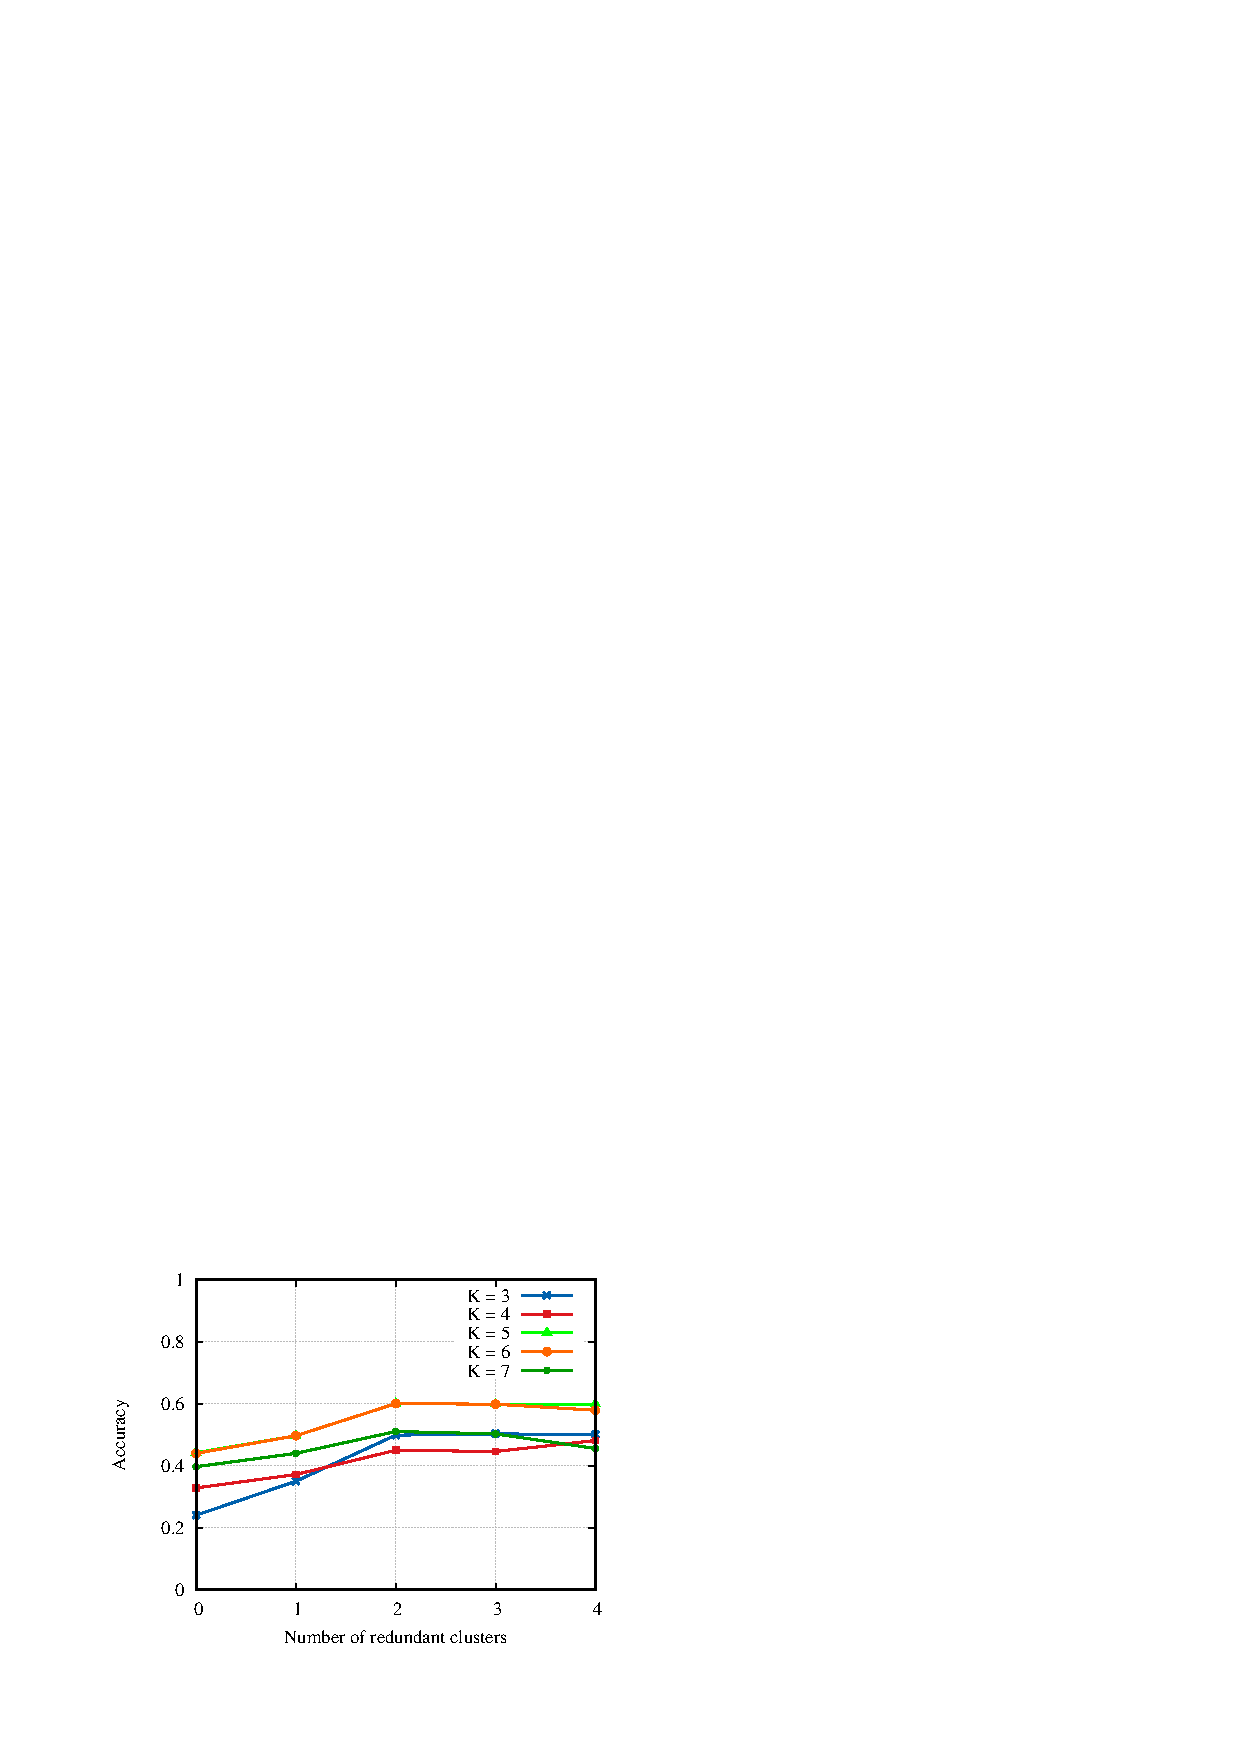
\includegraphics[width=0.8\columnwidth]{data/redundant_clusters_hotel}
		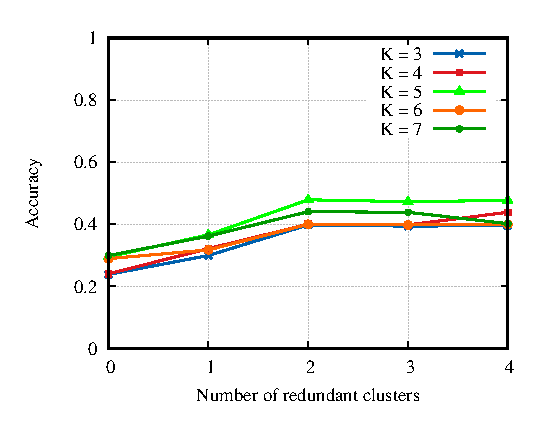
\includegraphics[width=0.8\columnwidth]{data/redundant_clusters_mobile}}
	\vfill
	\subfloat[The performance of different models when adjusting the number of 
	expected aspects $K$. Left: hotel reviews. Right: mobile phone reviews.
	\label{fig:differentk}]{
		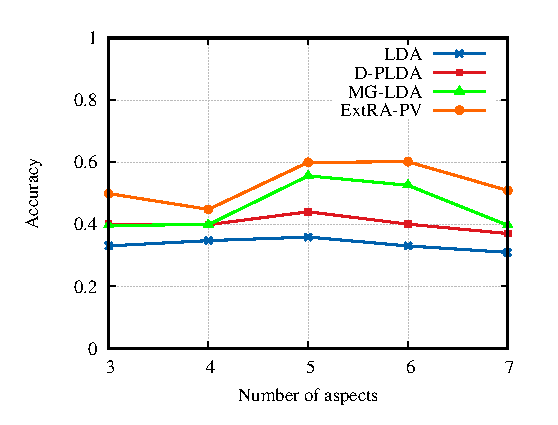
\includegraphics[width=0.8\columnwidth]{data/aspects_hotel}
		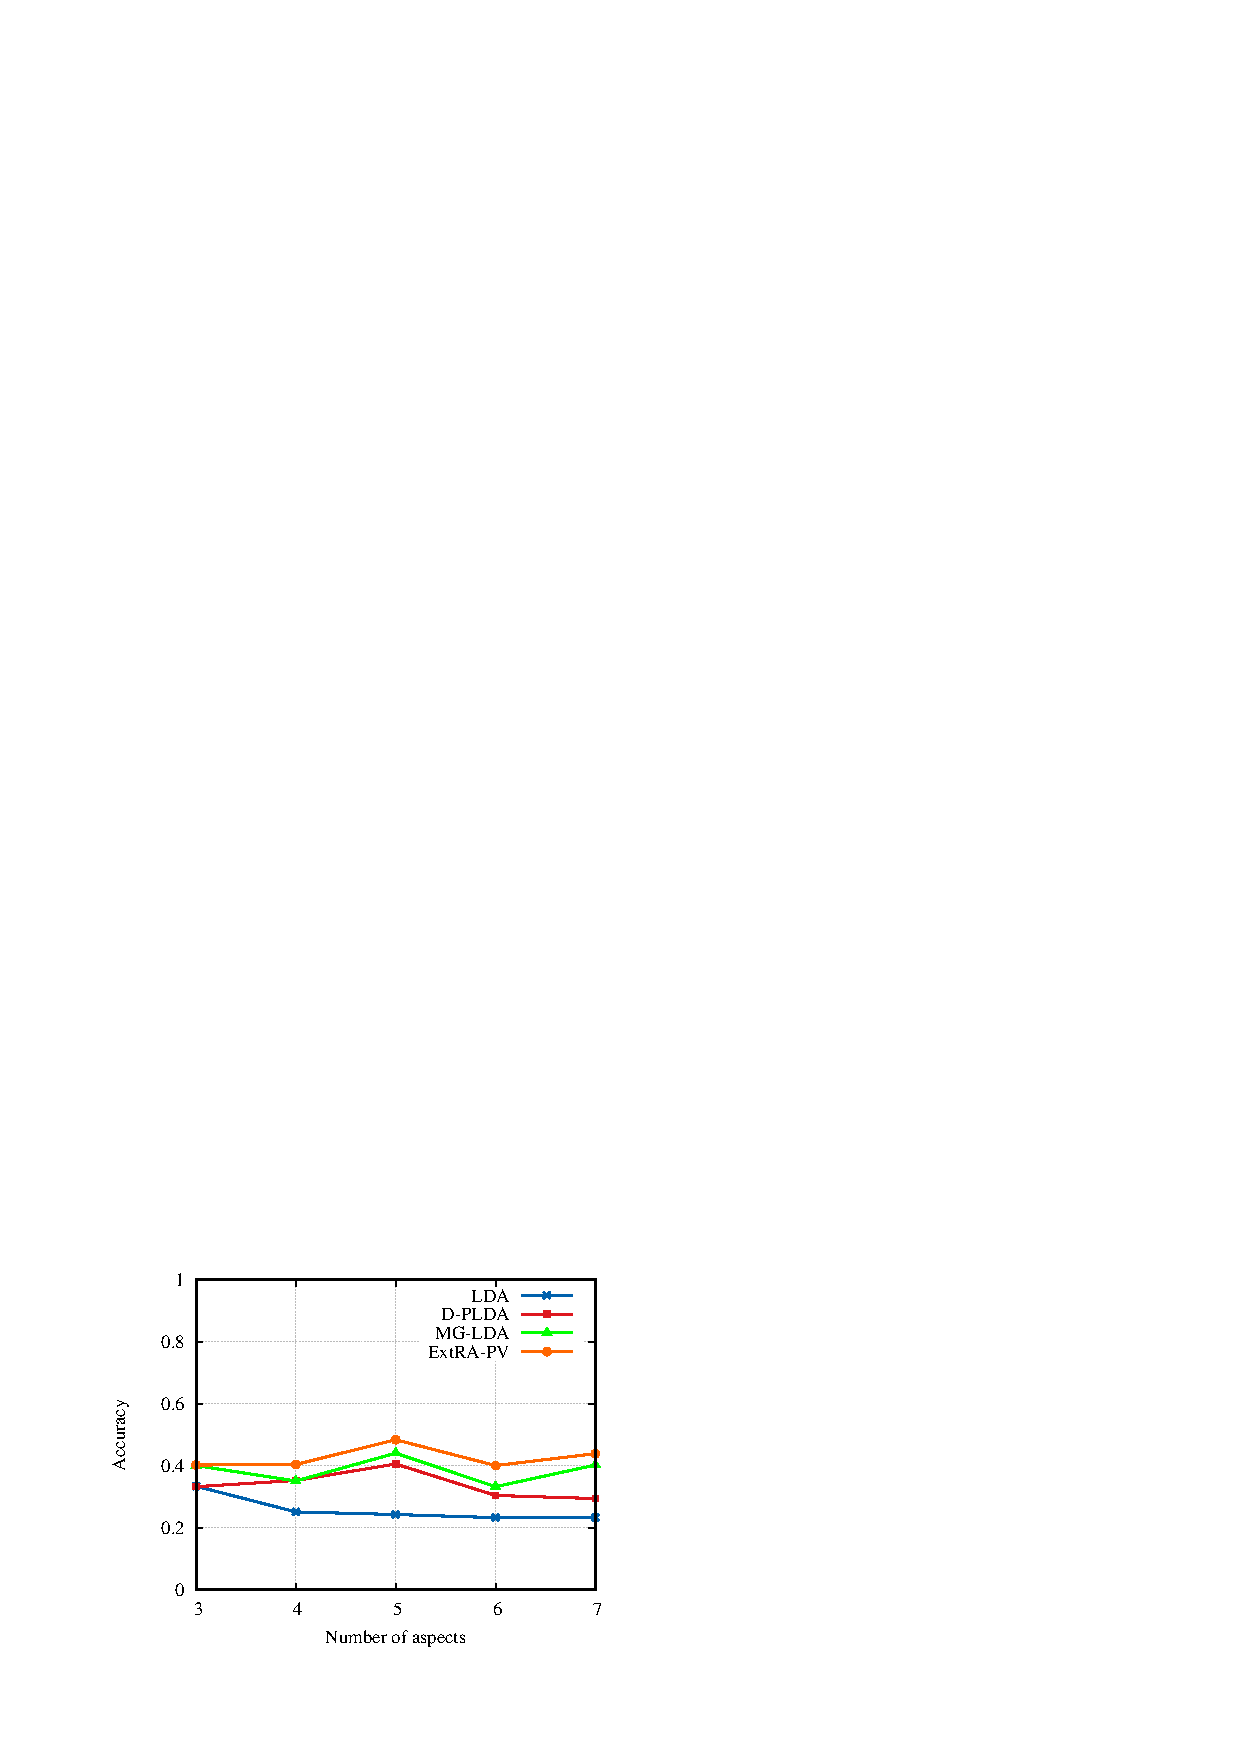
\includegraphics[width=0.8\columnwidth]{data/aspects_mobile}}
	\caption{Parameter Selection}
\end{figure*}
In this section we conduct experiments to determine the best set of
parameters of our model, most importantly the constants $N$, $M$, $C$.

\textbf{Number of Sentence Clusters ($N$)}

In the first clustering step we use a k-means to cluster the sentences,
where each cluster should contain sentences about similar aspects.
We need to determine the number of clusters, $N$.
We use an empirical elbow method to determine $N$, 
we plot the total distance between each point and its corresponding center,
a.k.a. the loss, with different choices of $N$, 
as shown in \figref{fig:differentn}.
Note that we don't concern about the number of expected aspects 
in this experiments. 
As we can see from \figref{fig:differentn},
to give the lowest loss, the number of sentence clusters should be
10 or 11.  Therefore, in the following experiments, we set $N$ to be 10.

\begin{figure}[th!]
\centering
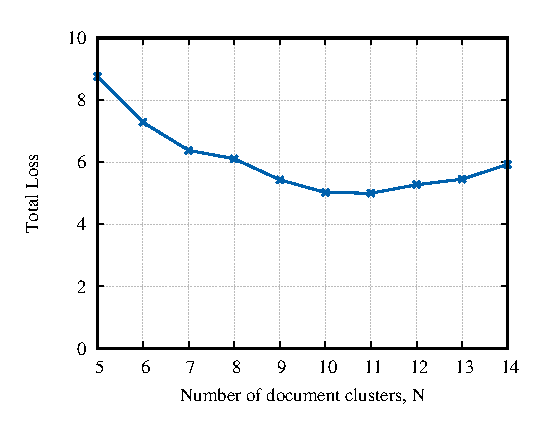
\includegraphics[width=0.8\columnwidth]{data/differentn}
\caption{Selecting $N$, the number of clusters for k-means. The optimal
$N$ is selected to be 10.}
\label{fig:differentn}
\end{figure}

\textbf{Number of LDA Topics ($M$)}

LDA in our model serves the purpose of isolating the 
noisy topics and resolving the overlaps between aspects.
In our experiments we find that different number of LDA topics
doesn't have much effect on the end-to-end performance.
As an example, the aspect extraction accuracy with different $M$
on hotel reviews are shown in \tabref{table:differentm}.
Consider the 25 manually annotated words again,
the difference between the three numbers is only 
1 out of 25 words.
In our experiments, $M$ is fixed to 10.
\begin{table}[th]
	\centering
	\caption{The effect of different number of LDA topics}
	\label{table:differentm}
	\begin{tabular}{|c|c|c|c|}
		\hline
		$M$ & 5 & 8 & 10 \\\hline
		Accuracy & 17/25 & 16/25 & 17/25 \\\hline
	\end{tabular}
\end{table}

\textbf{Redundant Clusters ($C$)}

As mentioned in \secref{sec:topic_clustering}, 
we generate $C$ aspect clusters before ranking the clusters and the words, where $C$ is larger than $K$.
In this section we demonstrate the effect of these redundant clusters.
In \figref{fig:differentc}, we show the accuracy with different 
redundancy $C-K$, 
ranging from 0 to 4, with number of expected aspects ranging from 3 to 7.
It can be seen that 2 redundant clusters are sufficient and 
more redundancies can't improve the performance.

\subsubsection{Models}

In this section we introduce the models used in our end-to-end comparison.
We compare 5 models in our experiments, 
LDA as a simple baseline, 
D-PLDA \cite{moghaddam2012design} as a representative for joint aspect-sentiment models, 
MG-LDA \cite{titov2008modeling} as a representative for aspect extraction topic models,
and two variations of our model, i.e. ExtRA-LSTM and ExtRA-PV. 
We run the 5 models on the review data for each product type separately. The number of aspects is fixed to 5.

\paragraph{LDA}
We use LDA as a simple topic model baseline. 
We treat each review as a document and run on the whole corpus (single product type). 
The number of topics is set to 5 for model comparison.

\paragraph{D-PLDA}
D-PLDA \cite{moghaddam2012design} is an LDA variation designed specifically for modeling user reviews. 
In D-PLDA, only opinion phrases are modeled, 
and the nouns and the phrases are controlled by two separate hidden parameters. There is a dependency from hidden parameter for adjectives to the one for nouns.
We use D-PLDA as a representative for models with join aspect and sentiment inference.


\paragraph{MG-LDA}
To compare our model with a popular, well-performed model designed for aspect extraction, 
we use MG-LDA \cite{titov2008modeling}. 
MG-LDA also models topics at different granularities. 
For model comparison, the number of local topics (aspect topics) is set to 5, 
the number of global topics is set to 30 (ignored in evaluation).

\paragraph{Our models}
\label{ourmodels}
For sentence vectors (both LSTM and PV), the dimensionality is set to 300.
We refer such models as ExtRA-PV and ExtRA-LSTM. Our framework can be extended to extract multi-word aspects by integrating AspVec, which is called ExtRA-PV+Phrase.
The number of sentence-level clusters is set to 10; the number of LDA topics is 10; the number of final word clusters in the clustering phase is 7 and is later reduced to 5 in the ranking phase. For training the sentence vectors, we do not use any extra data, all the word and sentence vectors are trained on the set of reviews for a single product type. 


\subsubsection{End-to-End Comparison}

%\begin{figure*}[t!]
%\centering
%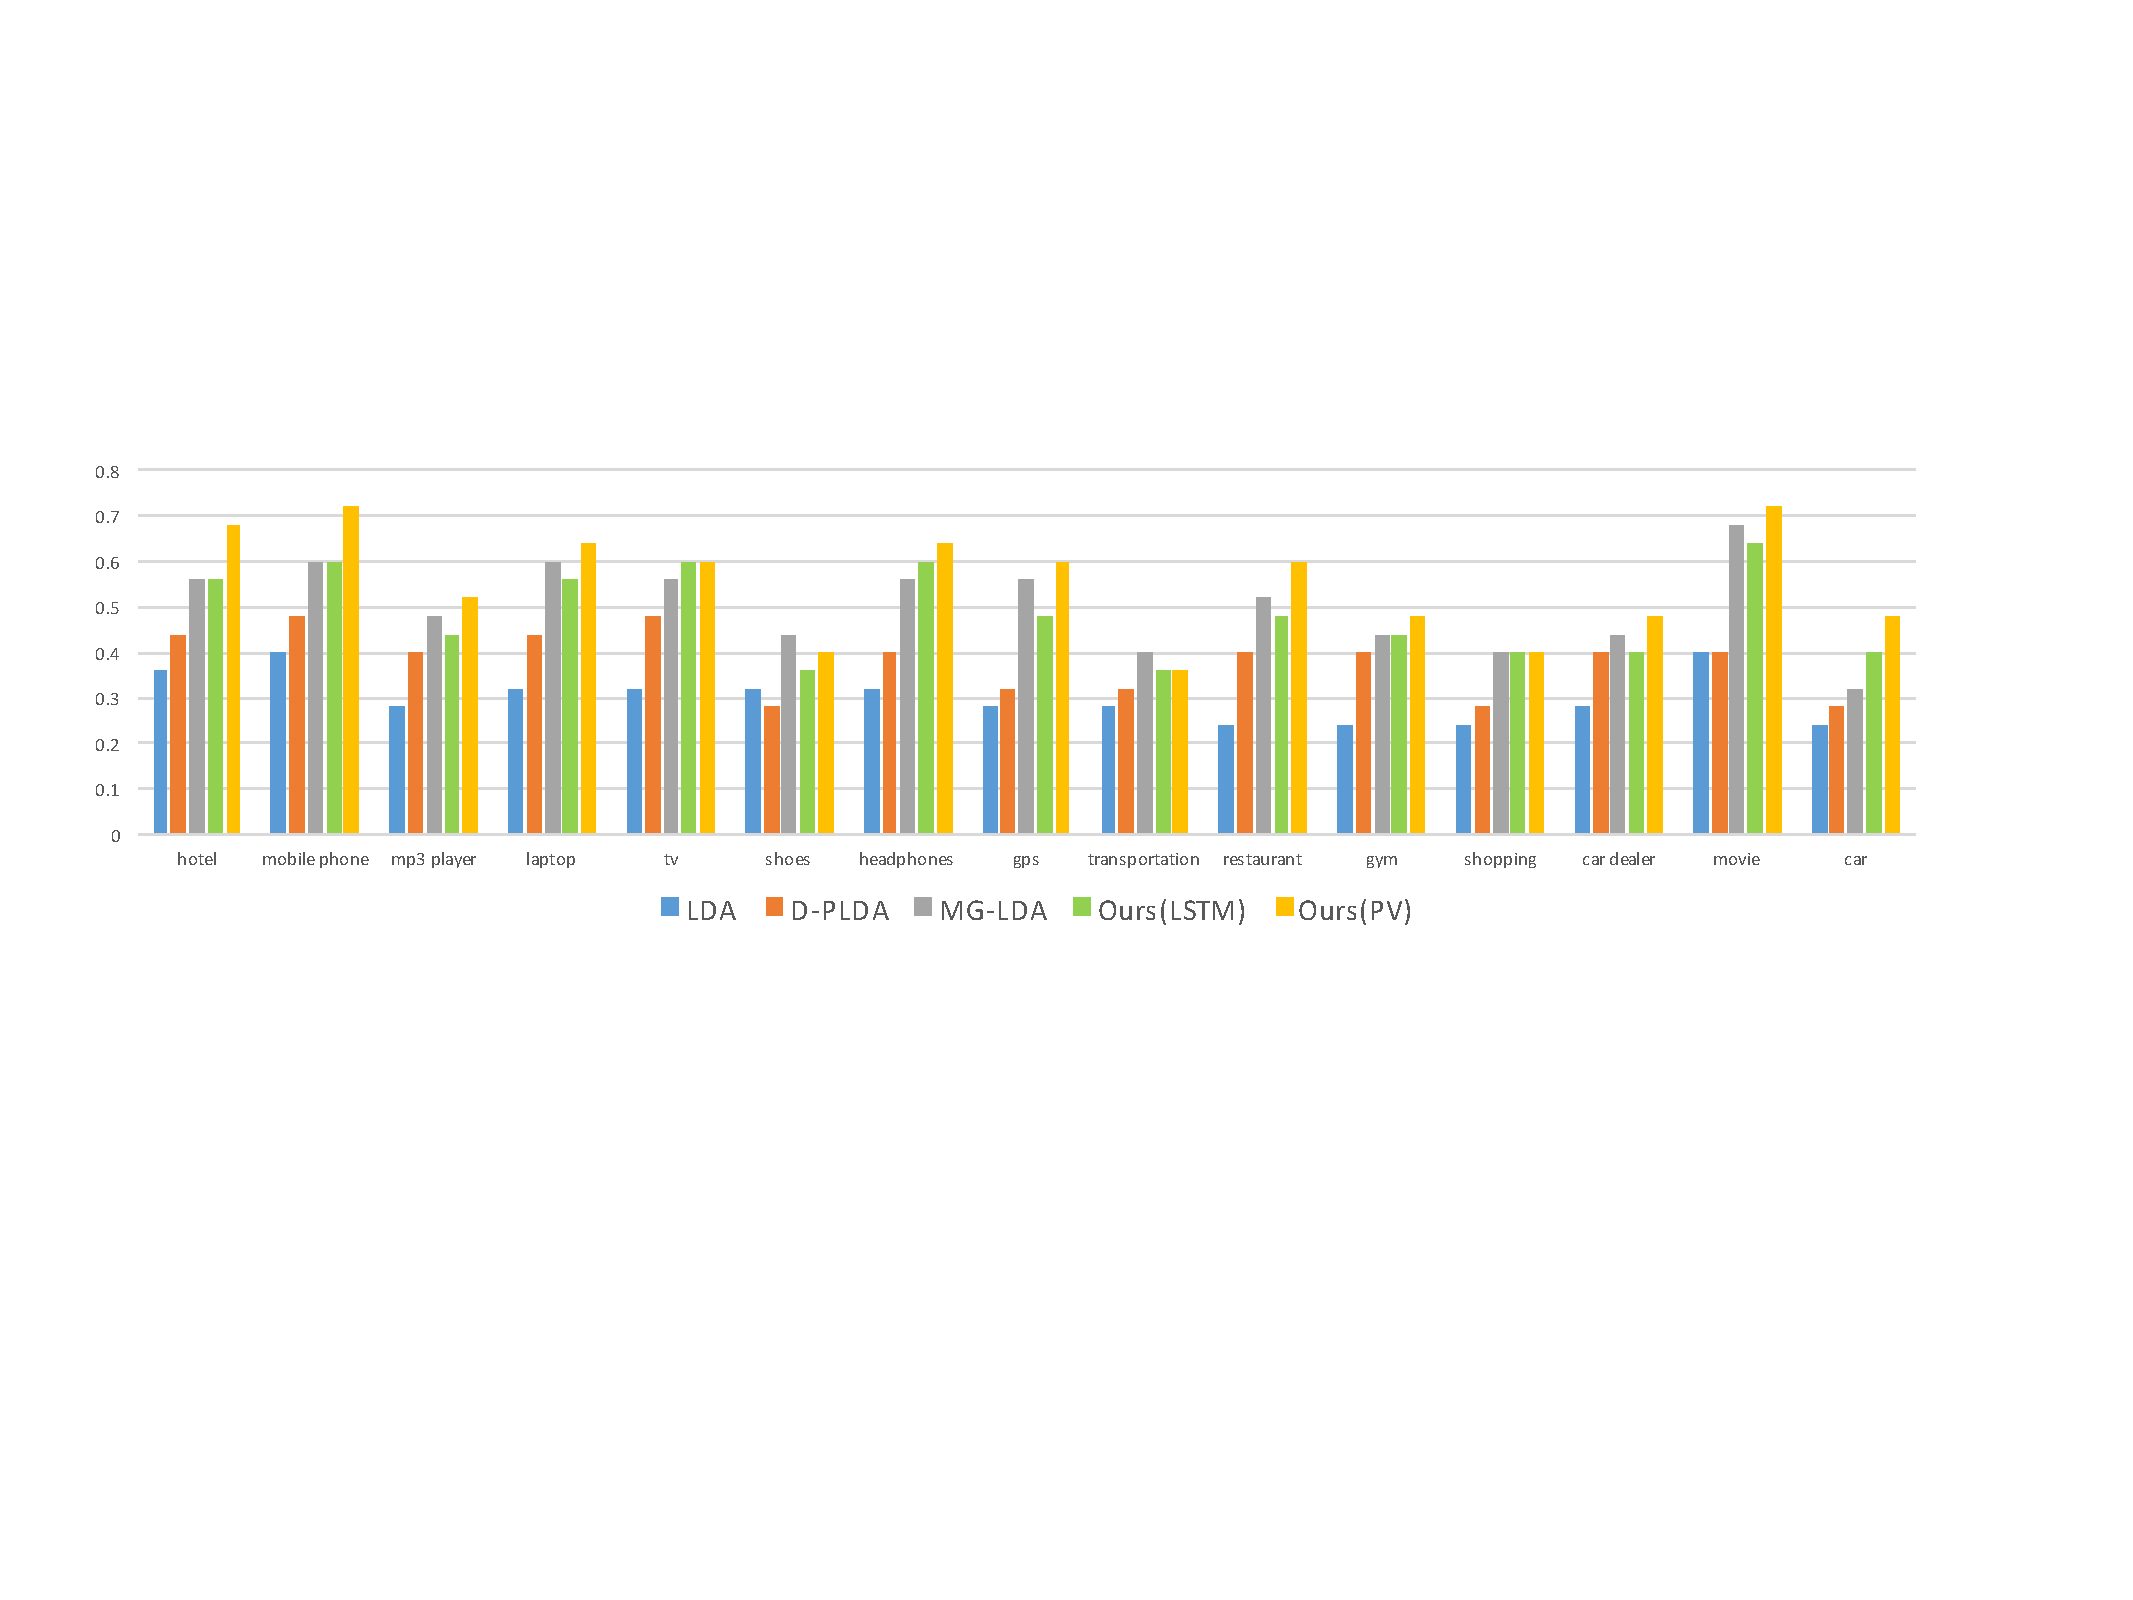
\includegraphics[width=2.0\columnwidth]{figures/results}
%\caption{Comparison of accuracies from different models on aspect extraction.}
%\label{fig:results}
%\end{figure*}


\begin{table}[th]
	\centering
	\caption{Comparison of accuracies using different models for aspect extraction.}
	\label{table:comparison}
	\begin{tabular}{|c|C{0.9cm}|C{0.9cm}|C{0.9cm}|C{0.9cm}|C{0.9cm}|}
		\hline
		\diagbox{Type}{Model}& LDA & D-PLDA & MG-LDA & ExtRA-LSTM & ExtRA-PV \\ \hline
		hotel &0.36 & 0.44 & 0.56 & 0.56 & \textbf{0.68} \\ \hline
		mobile phone & 0.40 & 0.48 & 0.60 & 0.60 & \textbf{0.72} \\ \hline
		mp3 player & 0.28 & 0.40 & 0.48 & 0.44 & \textbf{0.52} \\ \hline
		laptop & 0.32 & 0.44 & 0.60 & 0.56 & \textbf{0.64} \\ \hline
		camera & 0.34 & 0.43 & 0.62 & 0.55 & \textbf{0.62} \\ \hline
		restaurant & 0.24 & 0.40 & 0.52 & 0.48 & \textbf{0.60} \\ \hline
	\end{tabular}
\end{table}


In the end-to-end evaluation, we compare the performance of our models on aspect extraction with three other models as mentioned above. The results are shown in \tabref{table:comparison}. Our models outperform others in all of the categories. 
Our model with paragraph vector performs better than with LSTM, 
which is consistent to our result from the previous experiment.

We show the aspect word clusters on hotel reviews in \tabref{table:hotel_aspect_words}. The top words, which are chosen as the representatives of the aspects, are shown in boldface. 
\figref{fig:topiccloud} is the visualization (using TopicCloud toolkit\footnote{Open sourced toolkit is available at \url{https://github.com/askerlee/topiccloud}} \cite{li2017document}) for aspect clusters generated by ExtRA-PV+Phrase model on hotel review.
The portion of area for clusters depends on their distinctiveness score.
And the score of words in each cluster determines their size. With this visualization, the importance of each cluster and word is clearly shown, which makes comprehension easier. 


\begin{figure}[th]
	\centering
	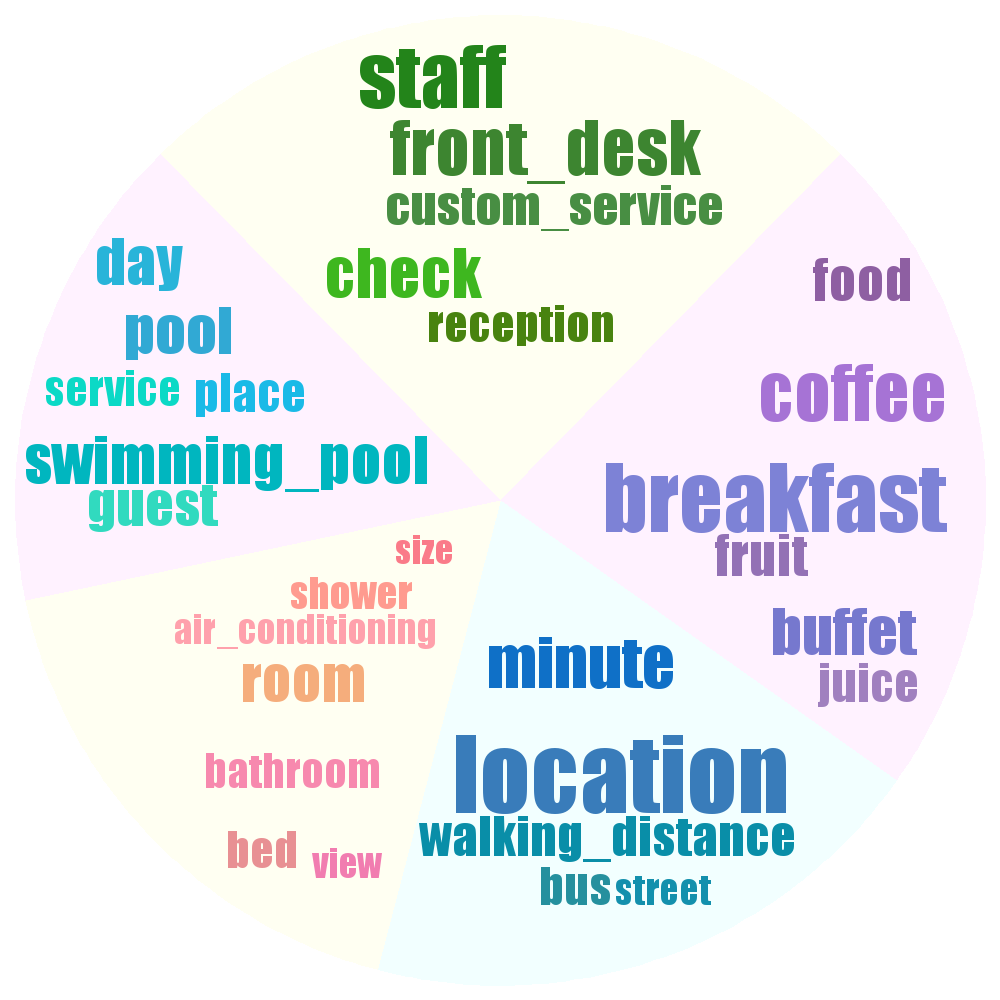
\includegraphics[width=0.8\columnwidth]{figures/topics_hotel}
	\caption{Aspect Cloud: visualization of aspect words and phrases extracted from the hotel reviews.}
	\label{fig:topiccloud}
\end{figure}

\begin{table}[th]
\centering
\caption{Top aspect words (with phrases) for hotel reviews by different models}
\label{table:hotel_aspect_words}
\begin{tabular}{|l|l|} \hline
\multirow{5}{*}{ExtRA-LSTM}
& \textbf{service}, front, desk, reception, concierge, check, gust \\
& \textbf{location}, station, minute, tube, station, bus, distance \\
& \textbf{time}, check, day, desk, charge, book, front, hour, night \\
& \textbf{food}, coffee, buffet, morning, tea, room, fruit, egg, juice \\
& \textbf{bed}, bathroom, size, floor, view, suite, king, book, decor \\ \hline

\multirow{5}{*}{ExtRA-PV}
& \textbf {staff}, service, room, front, desk, check, concierge \\
& \textbf {food}, breakfast, bar, restaurant, coffee, morning, tea \\
& \textbf {price}, parking, night, place, rate, service, money, star \\
& \textbf {room}, bed, bathroom, size, suite, floor, view, bedroom \\
& \textbf {location}, minute, square, subway, street, block, distance \\\hline

\multirow{5}{*}{ExtRA-PV+Phrase}
&  \textbf{staff}, front\_desk, check, custom\_service, reception, concierge \\
&  \textbf{breakfast}, coffee, buffet, food, fruit, juice, tea \\
&  \textbf{location}, minute, walking\_distance, bus, street, block \\
&  \textbf{room}, bed, bathroom, shower, air\_conditioning, view, size \\
&  \textbf{swimming\_pool}, pool, guest, place, service, day \\\hline

\multirow{5}{*}{MG-LDA}
& \textbf{shower}, bathroom, room, floor, area, bedroom, desk, tea \\
& \textbf{time}, day, room, check, front, desk, night, service \\
& \textbf{food}, bar, service, breakfast, restaurant, staff, taxi \\
& \textbf{room}, bed, floor, place, air, night, bathroom, noise \\
& \textbf{price}, business, service, star, internet, location, staff \\\hline

\multirow{5}{*}{DP-LDA}
& \textbf{service}, front, desk, reception, concierge, check, guest \\
& \textbf{station}, minute, tube, location, bus, distance, street \\
& \textbf{check}, day, time, desk, charge, book, front, hour \\
& \textbf{coffee}, buffet, morning, tea, room, day, fruit, food \\
& \textbf{bed}, bathroom, size, floor, view, suite, king, book \\\hline

\multirow{5}{*}{LDA}
& \textbf{stay}, night, place, trip, time, weekend, night, hour \\
& \textbf{location}, square, street, place, restaurant, market, block \\
& \textbf{room}, bed, bathroom, size, tv, king, suite, pillow \\
& \textbf{staff}, service, desk, location, concierge, room, night \\
& \textbf{room}, floor, noise, view, night, water, door, bathroom \\\hline
\end{tabular}
\end{table}


\subsubsection{Effect of Number of Expected Aspects ($K$)}


To evaluate the effect of different number of expected aspects, i.e. $K$, which 
determines the coverage covered by expected aspects,
we ask our annotators to provide different number of labels on two categories. 
The number of aspects range from three to seven. 
The performance of the four models when changing the number of aspects are shown in \figref{fig:differentk}. 
It can be seen that our models can well extract aspects with variant coverage and perform constantly better than all other models regardless of the number of expected aspects. 


\subsubsection{Effectiveness of Ranking}

Here we test the effectiveness of several techniques proposed for 
the ranking step.
In particular, we compare three setups:
\begin{itemize}
    \item No word ranking. 
          Use directly the word with highest score from aspect cluster after aspect inference. 
          Remove redundant clusters with cluster ranking.
    \item No duplicate prevention.
          As mentioned in \secref{sec:word_ranking}, we do duplicate prevention
          by considering other clusters when ranking words within a cluster.
          In this setup we do not include this effort.
    \item Use all ranking methods.
\end{itemize}


\begin{table}[th]
	\centering
	\caption{The accuracy performance with different ranking setups.}
	\label{table:rankingeffect}
	\begin{tabular}{|c|C{1.5cm}|C{1.5cm}|C{1.5cm}|}
		\hline
		\diagbox{Type}{Setup} & No word ranking & Word ranking w/o. duplicate prevention & Word ranking w. duplicate prevention \\ \hline
		hotel &0.48 &0.60 & \textbf{0.68} \\ \hline
		mobile phone &0.52 &0.64 & \textbf{0.72} \\ \hline
		mp3 player &0.36 & 0.44 & \textbf{0.52} \\ \hline
		laptop & 0.44 &0.52 & \textbf{0.64} \\ \hline
		camera & 0.43 &0.49 & \textbf{0.58} \\ \hline
		restaurant &0.48 &0.56 & \textbf{0.60} \\ \hline	
	\end{tabular}
\end{table}

%\begin{figure*}[th]
%	\centering
%	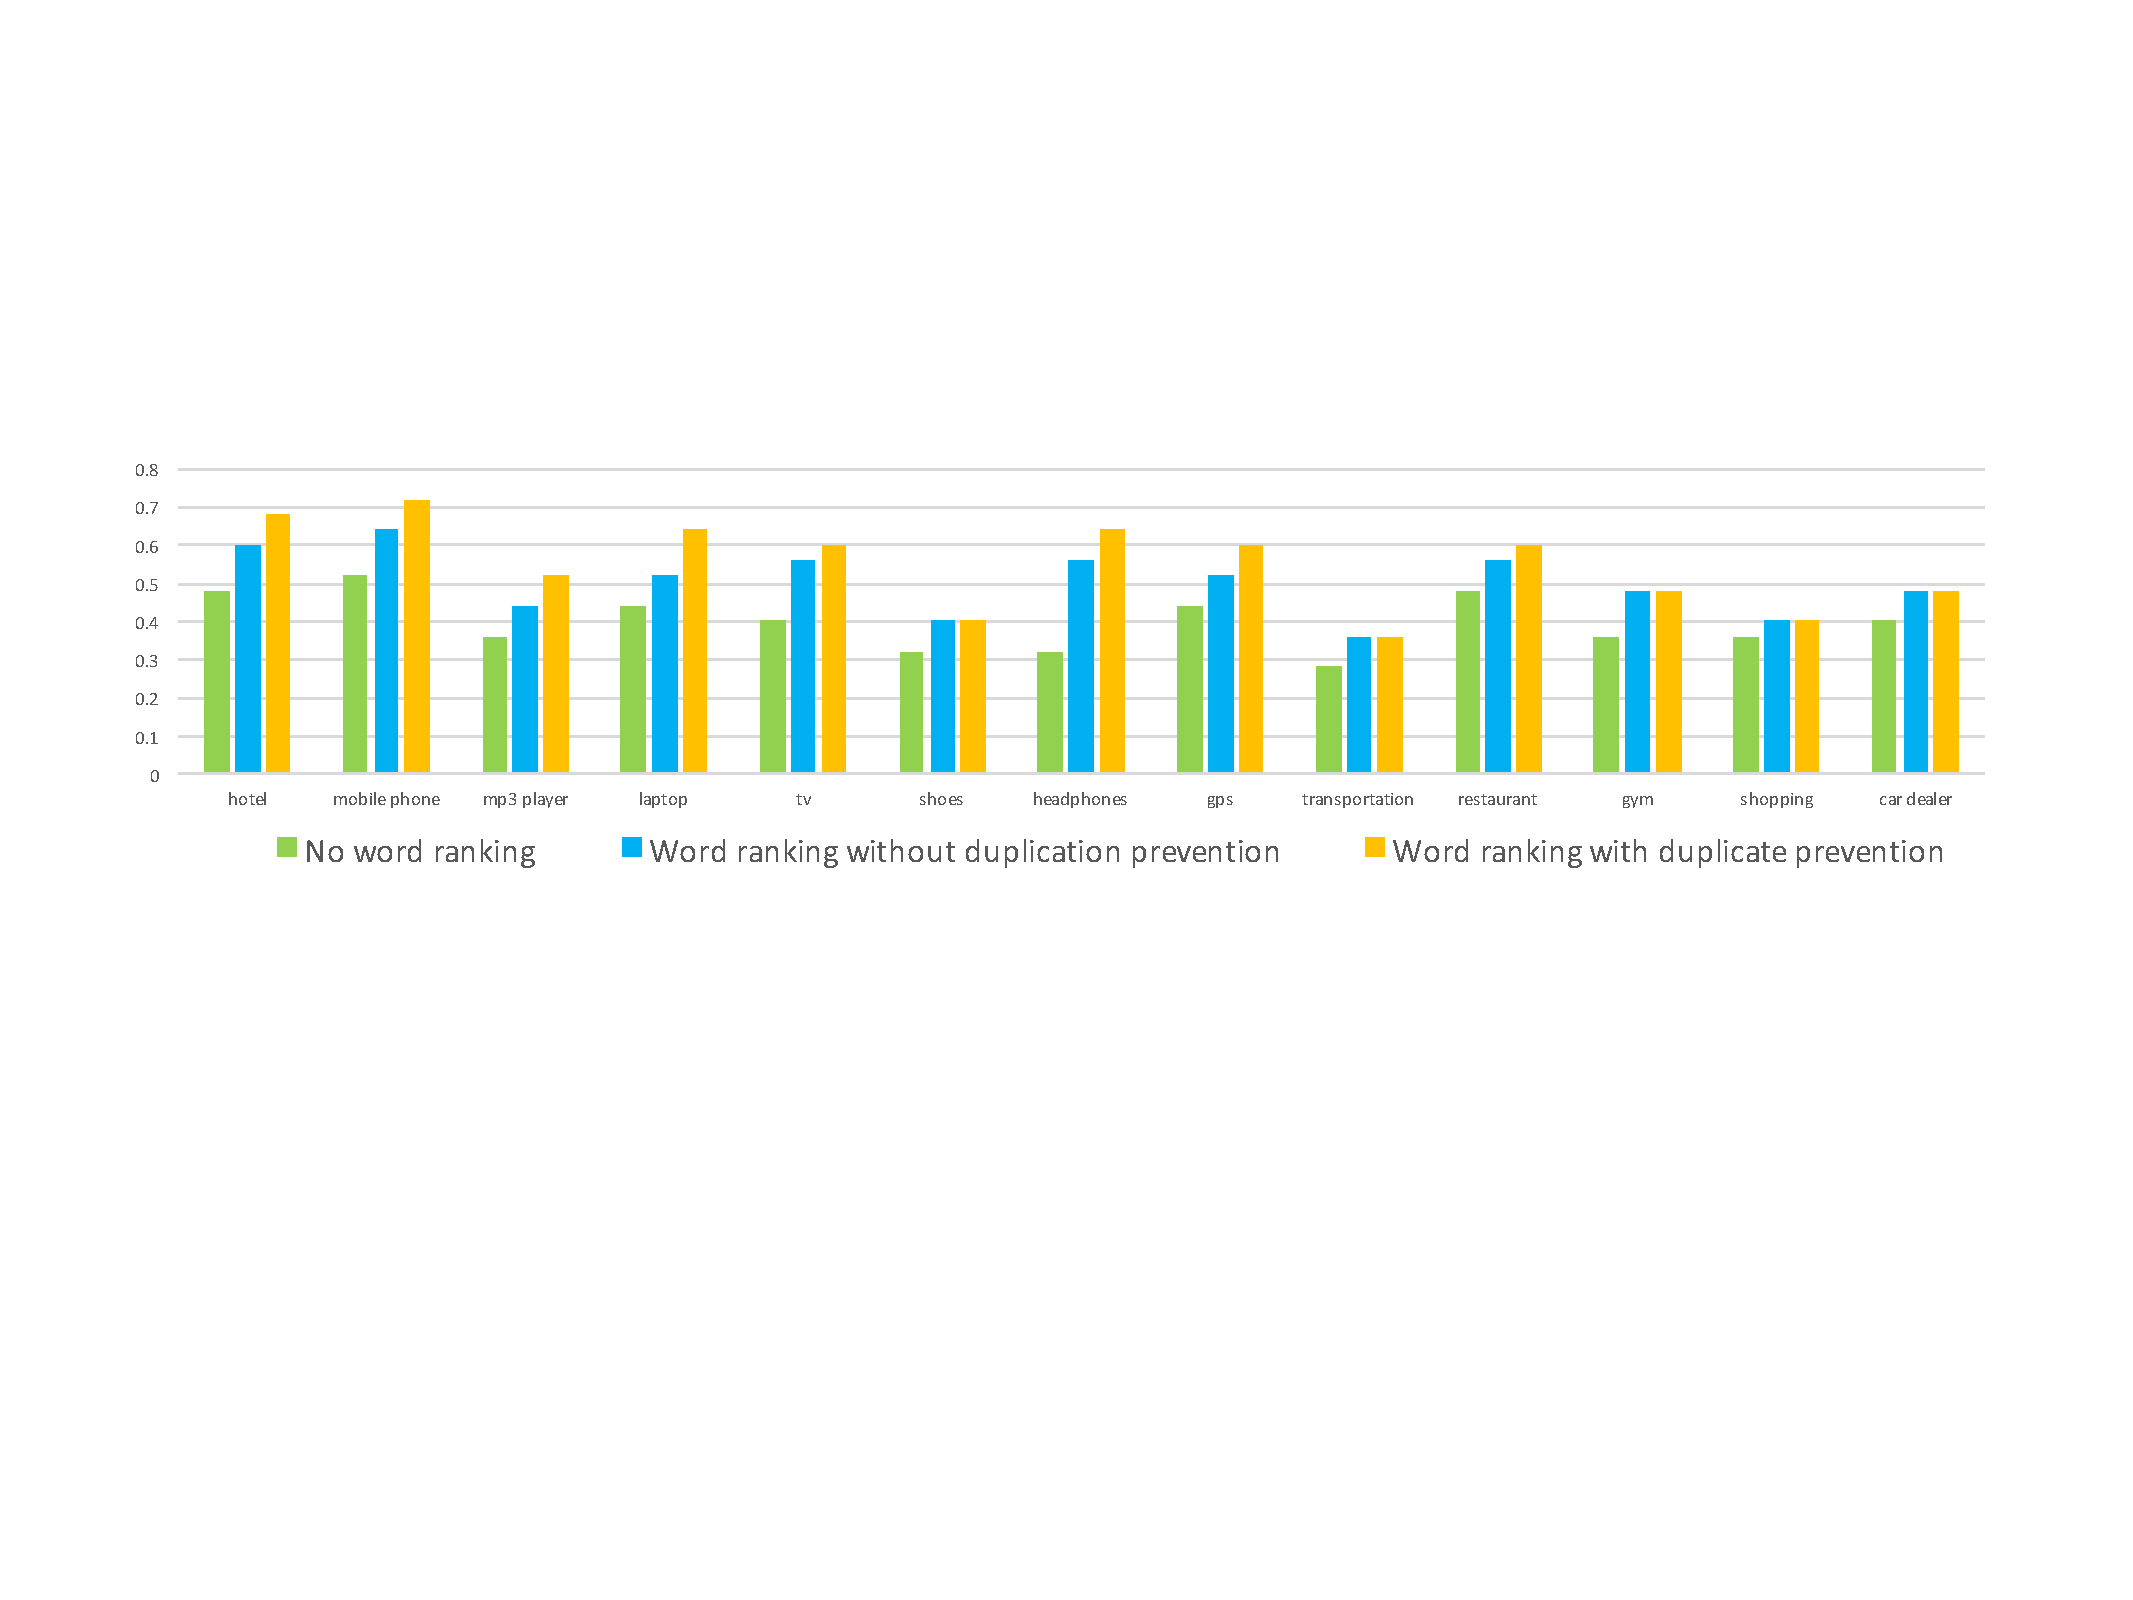
\includegraphics[width=2.0\columnwidth]{figures/rankingeffect}
%	\caption{The accuracy performance with different ranking setups.}
%	\label{fig:rankingeffect}
%\end{figure*}

The results are shown in \tabref{table:rankingeffect}.
The ranking scheme we propose, that is, word ranking with duplicate prevention,
has clear advantage across all product categories.

\subsection{Experiment 3: Aspect-based Review Summarization}
\label{sec:exp4}

In the last experiment, we present an end-to-end demo system\footnote{Our demo system is available at \url{http://anonymized.due.to.blind.review}} based on our proposed aspect extraction framework ExtRA. User can select a product type from a predefined set of categories, and sets the
number of aspects K. \figref{fig:experiments:sentimentcompare} shows an example about mobile phones. The aspect clusters by our method on the mobile phones review data is shown in \tabref{table:clusters}.  We use the top aspect words extracted by our model to represent clusters (in this example, we set $K=6$). The user may filter out some of the results by using the search box. The system demonstrates the review summaries of the selected products. Each summary contains the aspects and their scores. The scores are calculated according to the sentiment value of review sentences. To identify the aspects in the review sentences, we check if the top aspect words in each cluster appeared. 
If so, the sentiment value of the sentence for the identified aspects is predicted with an LSTM and feed-forward network model trained on Stanford Sentiment Treebank \cite{socher2013recursive}. The score for each aspect from the whole set is the average of the predicted sentiment values attached on it. With this system, users can easily compare different products with respect to the same set of important aspects, without having to read a lot of reviews. Comparison between Apple iPhone 6 and Samsung Galaxy S5 (see \figref{fig:experiments:sentimentcompare}) clearly indicates that Apple has better quality at the cost of less competitive price. Besides this concise format, sometimes users need much more details before their final decision. For this purpose, if the user wishes to understand why a product receives a score for a certain aspect, they can click on the ``xxx customer reviews'' link and be directed to the original review snippets with the aspect words and sentiment words highlighted (annotated using Stanford CoreNLP toolkit\cite{manning-EtAl:2014:P14-5}). The review snippets can be further grouped by aspects by clicking on the tabs(see \figref{fig:experiments:sentimentexample}).

 
\begin{table}[th]
	\centering
	\caption{The aspect clusters generated from mobile phone reviews}
	\label{table:clusters}
	\begin{tabular}{|l|}
		\hline
		\textbf{screen}, resolution, touch, display, color, picture \\ \hline
		\textbf{battery}, power, charge, day, cable, charger \\ \hline
		\textbf{quality}, break, day, build, buy, control \\ \hline
		\textbf{service}, buy, check, help, website, shipping \\ \hline
		\textbf{price}, money, worth, cost, charge, free \\ \hline
		\textbf{design}, color, metal, case, plastic, silver \\ \hline
	\end{tabular}
\end{table}


\begin{figure}[th]
\centering
\subfloat[Automatically generated 6 aspects for mobile phones\label{fig:experiments:sentimentcompare}]{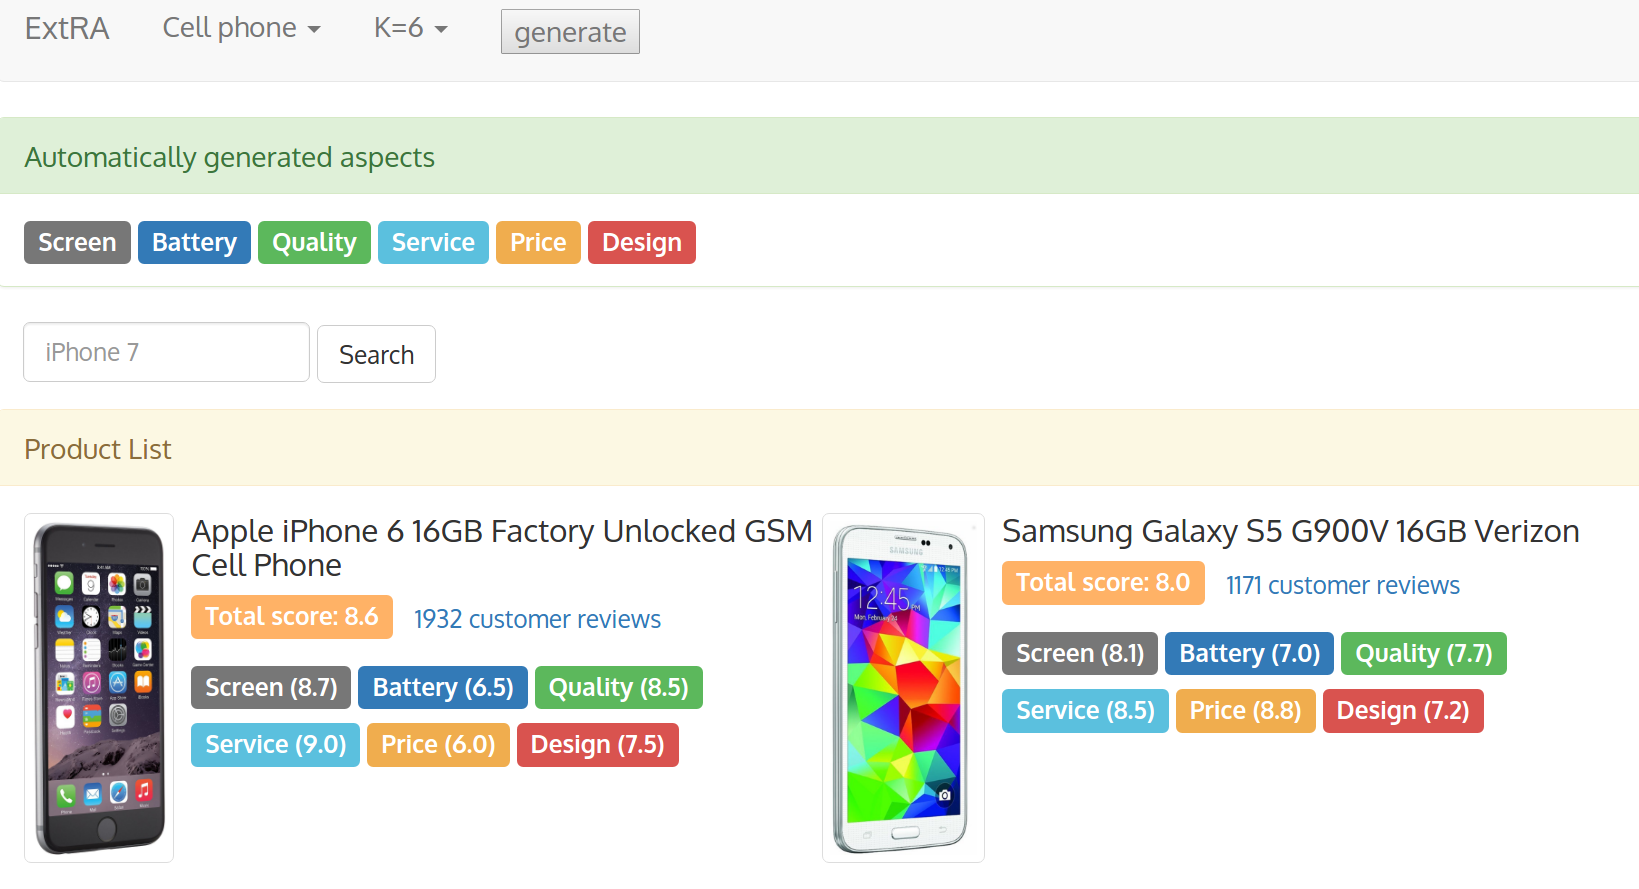
\includegraphics[width=1.0\columnwidth]{figures/sentimentcompare.png}}\vfill
\subfloat[Review snippets displayed by the aspects\label{fig:experiments:sentimentexample}]{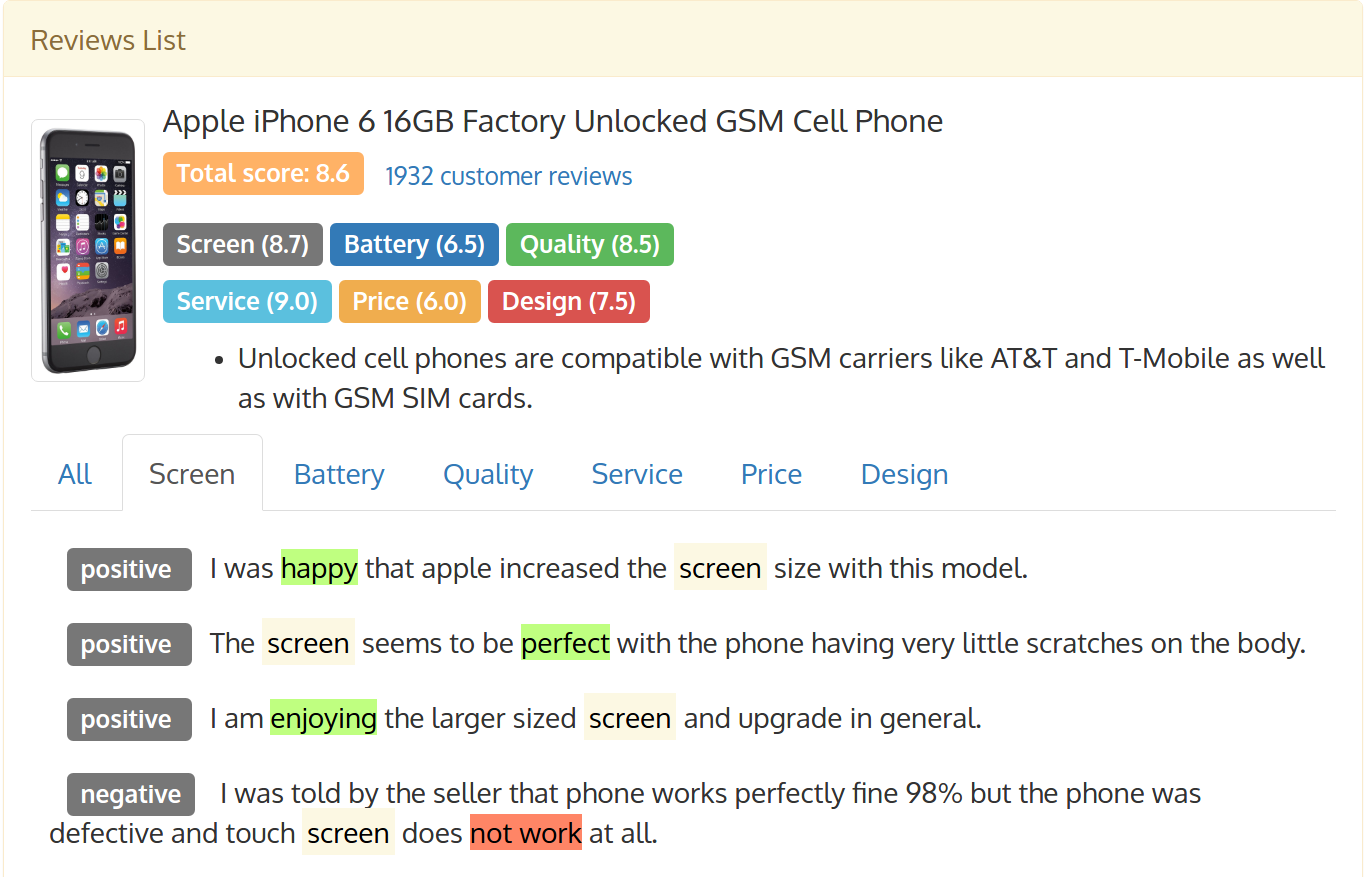
\includegraphics[width=1.0\columnwidth]{figures/sentimentexample.png}}
\caption{Demo system for ExtRA} \label{fig:experiments:sentimen}
\end{figure}


%
%In the last experiment,
%we demonstrate how to use our proposed aspect 
%extraction model to construct a complete aspect-based review summarization. 
%We use the top aspect words extracted by our model as the basis 
%for summarization, then predict the sentiment scores using a recurrent 
%neural network. Note that this summarization can be produced by 
%either a set of reviews or a single reivew. In this experiment, 
%we use our method to extract the aspects for mobile phones, 
%and produce aspect-based review summarization for 
%two different models of mobile phone, namely Samsung Galaxy Core Prime 
%and Apple iPhone 6.

%\begin{table}[th]
%	\centering
%	\caption{The aspect clusters generated from mobile phone reviews}
%	\label{table:clusters}
%	\begin{tabular}{|l|}
%		\hline
%		\textbf{screen}, resolution, touch, display, color, picture \\ \hline
%		\textbf{battery}, power, charge, day, cable, charger \\ \hline
%		\textbf{quality}, break, day, build, buy, control \\ \hline
%		\textbf{service}, buy, check, help, website, shipping \\ \hline
%		\textbf{price}, money, worth, cost, charge, free \\ \hline
%		\textbf{design}, color, metal, case, plastic, silver \\ \hline
%	\end{tabular}
%\end{table}
%
%The aspect clusters by our method on the mobile phone review data 
%is shown in \tabref{table:clusters}. Since the aspects are shared across 
%all the products within the same category, 
%we apply our model on the whole mobile 
%phone review dataset to extract these aspects. 
%Then we focus on the reviews for two specific models of mobile phone 
%and process them with a sentiment prediction backend.

%We use the aspect clusters shown in the above table to identify the 
%aspects in the review sentences by checking if the top aspect words 
%in each cluster appeared. If so, the sentence is attached with weight 
%equal to the highest aspect score it contains. Further, the sentiment 
%value of the sentence is predicted with an LSTM and feed-woward network 
%model trained on Stanford Sentiment Treebank \cite{socher2013recursive}. 
%The sentiment value for each aspect from the whole set is the 
%weighted average of the predicted sentiment values.

%The final aspect-based review summarization of two different mobile phones 
%are shown in \figref{fig:experiments:comparison}. 
%With this summarization, users can easily compare different products 
%with respect to the same set of important aspects, without having to 
%read a lot of reviews.

%\begin{figure}[th]
%\centering
%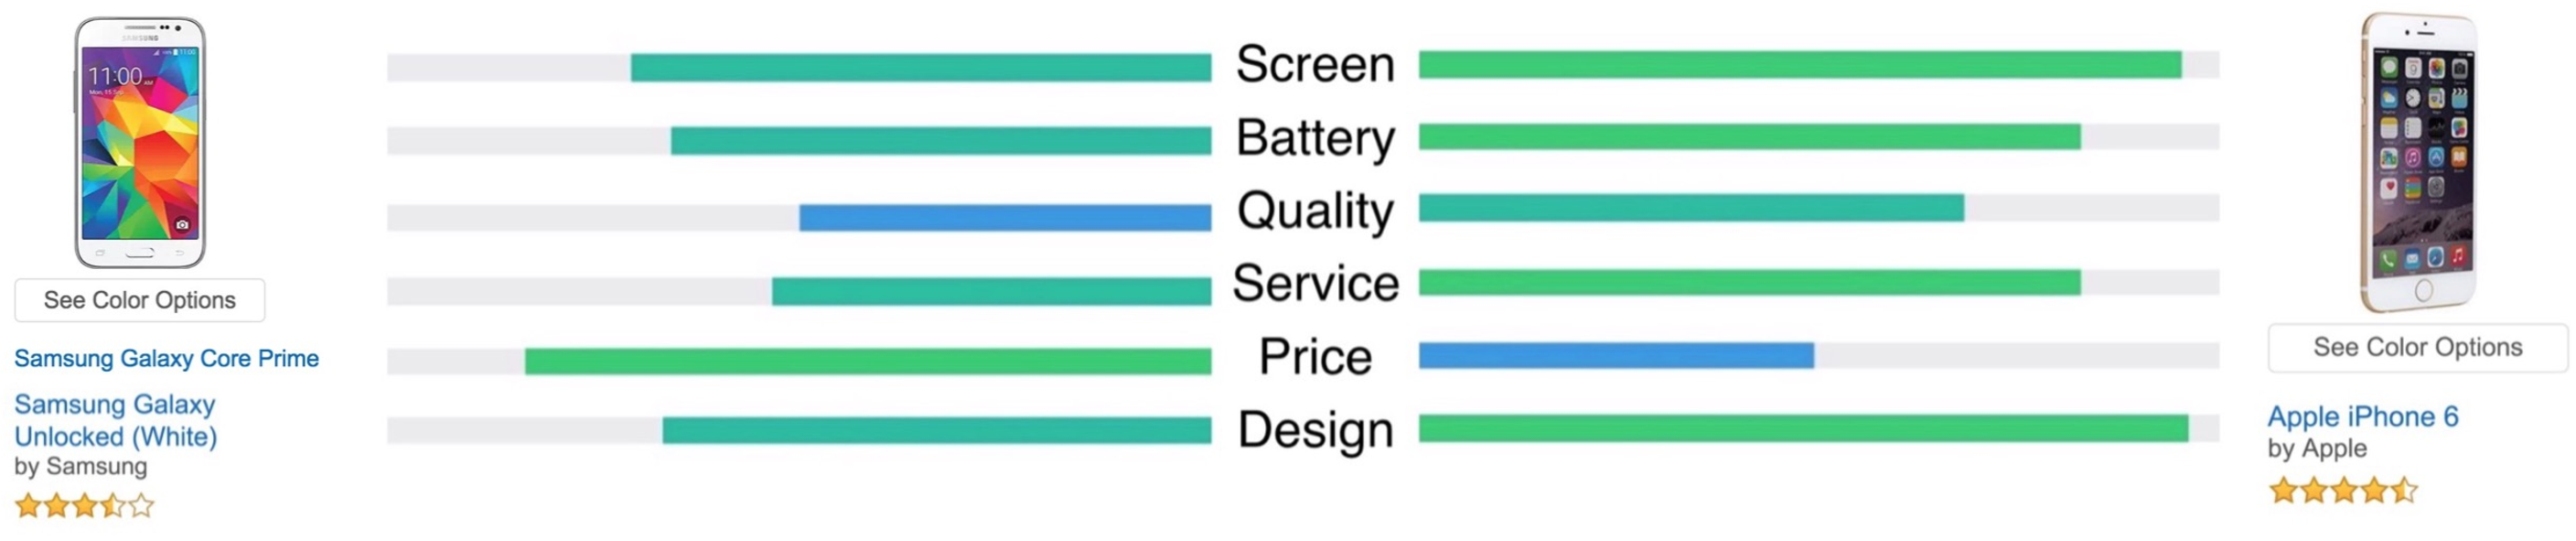
\includegraphics[width=1.0\columnwidth]{figures/comparison}
%\caption{Comparing two mobile phones.}
%\label{fig:experiments:comparison}
%\end{figure}

%\KZ{Where should the following para go? Doesn't seem very relevant to
%experiment 3. Is it a summary of the whole section? Then shouldnt start
%with Another...}
%One of the advantages of using our method for review summarization
%is that the chosen aspects 
%reflect what the consumers care most about each product type. 
%The fundamental reason behind this is that our model can truly leverage 
%the large amount of data compared to traditional methods. 
%In \figref{fig:phrases}, we can see phrases such as ``beautiful screen'' 
%and ``good camera'', but we also see ``high resolution'', which 
%is confusing because we cannot know if it means the screen or the camera, 
%and either way there is overlap in meaning. In our method, the topics of 
%the sentence is implicitly embedded in the sentence vector in the first 
%clustering process, so we can leverage not only the opinion phrases 
%but other surrounding words to decide whether ``high resolution'' 
%refers to the screen or the camera. For example, if the review 
%sentence is ``it has high resolution and the texts look so crisp'', 
%we would know it's about the screen. This allows our summarization to 
%leverage a lot more data than these traditional methods. 
